\documentclass[border=5mm,tikz]{standalone}
\usepackage{amssymb}
\usepackage{pgfplots}
%\usepgfplotslibrary{patchplots}
\usetikzlibrary{patterns, positioning, arrows}
\pgfplotsset{compat=1.15}
%\newcommand{\circo}{~\raisebox{1pt}{\tikz \draw[line width=0.5pt] circle(1.0pt);}~}

\begin{document}
    
    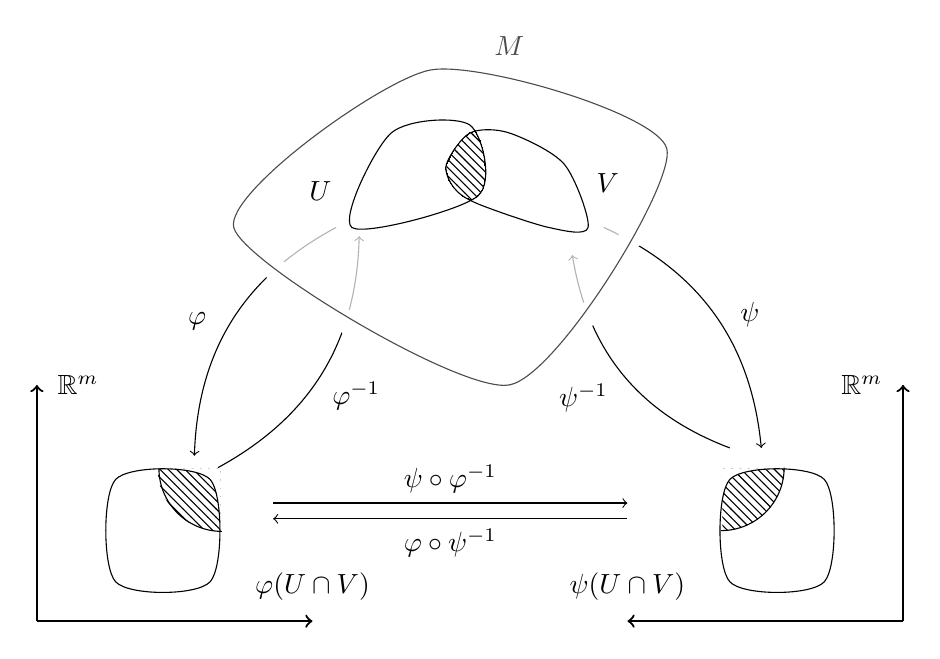
\begin{tikzpicture}
        
        % Functions i
        \path[->] (0.8, 0) edge [bend right] node[left, xshift=-2mm] {$\varphi$} (-1, -2.9);
        \draw[white,fill=white] (0.06,-0.57) circle (.15cm);
        \path[->] (-0.7, -3.05) edge [bend right] node [right, yshift=-3mm] {$\varphi^{-1}$} (1.093, -0.11);
        \draw[white, fill=white] (0.95,-1.2) circle (.15cm);
        
        % Functions j
        \path[->] (5.8, -2.8) edge [bend left] node[midway, xshift=-5mm, yshift=-3mm] {$\psi^{-1}$} (3.8, -0.35);
        \draw[white, fill=white] (4,-1.1) circle (.15cm);
        \path[->] (4.2, 0) edge [bend left] node[right, xshift=2mm] {$\psi$} (6.2, -2.8);
        \draw[white, fill=white] (4.54,-0.12) circle (.15cm);
        
        % Manifold pattern=north west lines,
        \draw[smooth cycle, tension=0.4, fill=white, pattern color=brown,  opacity=0.7] plot coordinates{(2,2) (-0.5,0) (3,-2) (5,1)} node at (3,2.3) {$M$};
        
        % Help lines
        %\draw[help lines] (-3,-6) grid (8,6);
        
        % Subsets
        \draw[smooth cycle, pattern color=orange] %, pattern=crosshatch dots] 
        plot coordinates {(1,0) (1.5, 1.2) (2.5,1.3) (2.6, 0.4)} 
        node [label={[label distance=-0.3cm, xshift=-2cm, fill=white]:$U$}] {};
        \draw[smooth cycle, pattern color=blue] %, pattern=crosshatch dots] 
        plot coordinates {(4, 0) (3.7, 0.8) (3.0, 1.2) (2.5, 1.2) (2.2, 0.8) (2.3, 0.5) (2.6, 0.3) (3.5, 0.0)} 
        node [label={[label distance=-0.8cm, xshift=.75cm, yshift=1cm, fill=white]:$V$}] {};

        \draw[line width=0.0mm,opacity=1,black, pattern color=black, pattern=north west lines] 
        plot coordinates { (2.57, 1.232)(2.5,1.2) (2.4,1.12)(2.3,1)(2.2, 0.8)(2.19,0.75)
            (2.21,0.68)(2.22,0.65)(2.23,0.61)(2.24,0.59)
             (2.3, 0.5)(2.4,0.4) (2.52,0.35) (2.55,0.37) (2.6,0.4) (2.67,0.5) (2.69,0.6)(2.7,0.7)
         (2.69,0.8)(2.68,0.9)(2.66,1.0)(2.63,1.1)(2.58,1.2)(2.57, 1.232)} {};

        
        % First Axis
        \draw[thick, ->] (-3,-5) -- (0.5, -5) node [label=above:$\varphi(U \cap V )$] {};
        \draw[thick, ->] (-3,-5) -- (-3, -2) node [label=right:$\mathbb{R}^m$] {};
        
        % Arrow from i to j
        \draw[->] (0, -3.5) -- node[midway, above]{$\psi \circ \varphi^{-1}$} (4.5, -3.5);
        \draw[<-] (0, -3.7) -- node[midway, below]{$\varphi\circ \psi^{-1}$} (4.5, -3.7);
        
        % Second Axis
        \draw[thick, <-] (4.5, -5)node [label=above:$\psi(U \cap V)$] {} -- (8, -5) ;
        \draw[thick, ->] (8, -5) -- (8, -2) node [label=left:$\mathbb{R}^m$] {};
        
        % Sets in R^m
        \draw[line width=0.01mm,white, pattern color=black, pattern=north west lines] (-0.67, -3.06) -- +(180:0.8) arc (180:270:0.8);
        \fill[even odd rule, white] [smooth cycle] plot coordinates{(-2, -4.5) (-2, -3.2) (-0.8, -3.2) (-0.8, -4.5)} (-0.67, -3.06) -- +(180:0.8) arc (180:270:0.8);
        \draw[smooth cycle] plot coordinates{(-2, -4.5) (-2, -3.2) (-0.8, -3.2) (-0.8, -4.5)};
        \draw (-1.45, -3.06) arc (180:270:0.8);
        
        \draw[white, pattern color=black, pattern=north west lines] (5.7, -3.06) -- +(-90:0.8) arc (-90:0:0.8);
        \fill[even odd rule, white] [smooth cycle] plot coordinates{(7, -4.5) (7, -3.2) (5.8, -3.2) (5.8, -4.5)} (5.7, -3.06) -- +(-90:0.8) arc (-90:0:0.8);
        \draw[smooth cycle] plot coordinates{(7, -4.5) (7, -3.2) (5.8, -3.2) (5.8, -4.5)};
        \draw (5.69, -3.85) arc (-90:0:0.8);
        
    \end{tikzpicture}
    
\end{document}